\chapter{Fundamentação Teórica}
\label{chp:fundamentaçãoTeórica}


\section{Propriedade Intelectual}

De acordo com \citet{WIPO2016} e \citet{howe2013concepts} o conceito de Propriedade Intelectual é definido como uma categoria de propriedade, que inclui criações intangíveis do intelecto humano, seja nos domínios industrial, científico, literário ou artístico. Por meio de leis é garantido aos responsáveis ou inventores quaisquer produção feita por eles.

A \ac{ompi} ou \textit{\ac{wipo}}\footnote{WIPO <https://www.wipo.int/portal/en/index.html> 
} divide a Propriedade Intelectual em três segmentos principais: os  direitos  autorais,  os  de Propriedade  Industrial,  e  outros  direitos  sobre  bens  imateriais  de  vários  gêneros (Proteção \textit{Sui Generis}\footnote{Os tipos de proteção sui generis abrangem desde as cultivares, as topografias de circuito integrado e os conhecimentos tradicionais;}),  conforme  ilustra \autoref{fig:PI}.

\begin{figure}[H]
\centering
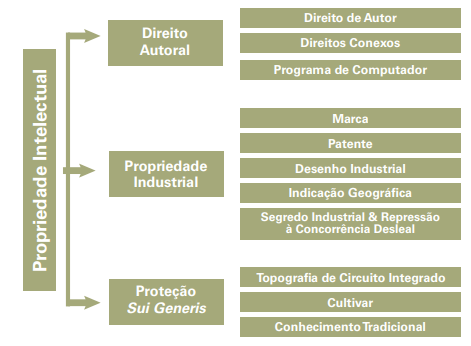
\includegraphics[]{images/modalidades}
\caption{Fonte: \citep{jungman2010}}
\label{fig:PI}
\end{figure}

Segundo \citet{buainain2005propriedade}, a propriedade intelectual:%definição
\begin{quote}
    "Possibilita transformar o conhecimento, em princípio um bem quase público, em bem privado e é o elo de ligação entre o conhecimento e o mercado."
\end{quote}

A razão da existência dos direitos à propriedade intelectual é impedir o uso não autorizado, a venda, fabricação ou importação de um produto similar na esfera de sua proteção de acordo com as leis vigentes. Justamente para que pessoas de má fé não tirem proveito do direito alheio.


\subsection{Lei Brasileira sobre \ac{pi}} 
No Brasil, existe uma lei específica que trata do assunto de propriedade intelectual, onde se dispõe sobre a proteção da propriedade intelectual de programa de computador, sua comercialização no país, além de mostrar providências relacionadas ao assunto. 

A proteção  é a mesma dada às obras literárias pela lei que trata dos direitos autorais. Além dessa lei, há uma legislação específica que trata do assunto: a Lei nº 9.609, de 19 de fevereiro de 1998, conhecida como Lei do Software\footnote{Disponível em: <http://www.planalto.gov.br/civil\_03/leis/L9609> Acesso em 17 mar. 2020}. %precisa referenciar no final?

O site do Instituto Nacional da Propriedade Industrial, afirmando o Decreto de Berna \citep{leideBerna} diz que: 

\begin{quote}
    "O registro de programa de computador é válido por 50 anos a partir da sua criação ou de 1º de janeiro do ano subsequente à sua publicação. A proteção não é territorial, isto é, sua abrangência é internacional, compreendendo os 175 países signatários da Convenção de Berna (1886)." \footnote{Fonte: <http://www.inpi.gov.br/servicos/perguntas-frequentes-paginas-internas/perguntas-frequentes-programa-de-computador>. Acessado em: 19 mar. 2020} \citep{leideBerna}
\end{quote}


A Lei de Direito Autoral (Lei nº 9.610/1998)\footnote{Fonte: <http://www.planalto.gov.br/ccivil\_03/leis/L9610.htm>. Acessado em: 19 mar. 2020}", juntamente com a Lei de Software (Lei nº 9.609/1998)", garantem proteção ao programa de computador em si, à expressão literal do software, isto é, suas linhas de código-fonte. Ao registrar o programa de computador no IMPI, obtém-se as garantias jurídicas necessárias para proteger o autor daquele código-fonte, inclusive, por exemplo, em situações de uma demanda judicial para comprovar a autoria ou titularidade do programa.

Não existe limitações com relação à quantidade de registros sobre um mesmo software e suas diferentes versões. Assim é possível garantir a máxima extensão para a proteção ao código-fonte. \citep{inpiPerguntasFrequentes} 

\begin{quote}
    "Aqui vale uma ressalva: softwares apenas conceituais, ou seja, programas de computador que ainda se encontrem meramente no campo da ideia, não são passíveis de proteção." \citep{inpiPerguntasFrequentes}
\end{quote}

Portanto implementações conceituais, precisam estar documentadas e implementadas, mesmo que de forma incompleta, para que seja validados os seus registros. 

Quanto o desenvolvimento do software está associado a uma relação de trabalho ou prestação de serviço, a indicação na lei é que os direitos relativos ao programa pertencem ao empregador, contratante ou órgão público, salvo quando há uma disposição contrária, quando o acordo contratual define. \citep{lei9609/98}

Assim de acordo com o artigo 28 da Lei 9.610/98 
\begin{quote}
    cabe ao Autor, ou ao detentor dos direitos autorais patrimoniais o direito exclusivo de utilizar, fruir e dispor da obra literária, artística ou científica”; \citep{lei9610/98}
\end{quote}“ 
e o artigo 29 da mesma lei
\begin{quote}
    “depende de autorização prévia e expressa do mesmo para que a obra seja utilizada, por quaisquer modalidades, dentre elas a reprodução parcial ou integral”. \citep{lei9610/98}
\end{quote}
Toda cópia reproduzida de forma não autorizada constitui de um ato ilícito civil e criminal, passível de punição de acordo com a lei brasileira.

\subsection{Licenças de Código Aberto  e Software Livre}

Existem iniciativa importantes que visam flexibilizar restrições e proteções relativas aos direitos autorais, são conhecidas como iniciativas de Código Aberto (do inglês \textit{"Open Source"} e o Software Livre. São iniciativas distintas que baseiam em conceder aos usuários liberdade para executar, copiar, distribuir e modificar o software, sem que haja transgressão aos direitos autorais.


De acordo com o site da GNU, software livre é definido como o respeito à liberdade e o senso de comunidade existente entre os usuários, dando liberdade para executar, copiar, distribuir, estudar e/ou melhorar o software. Algo que deve ser ressaltado é o fato do software livre não ser confundido com software grátis, são conceitos diferentes, onde alguns softwares livres podem ser gratuitos. \citep{gnu}

\begin{quote}
"Um programa é software livre se os usuários possuem as quatro liberdades essenciais:
\begin{itemize}
    \item liberdade de executar o programa como você desejar, para qualquer propósito (liberdade 0).
    \item liberdade de estudar como o programa funciona, e adaptá-lo às suas necessidades (liberdade 1). Para tanto, acesso ao código-fonte é um pré-requisito.
    \item liberdade de redistribuir cópias de modo que você possa ajudar outros (liberdade 2).
    \item liberdade de distribuir cópias de suas versões modificadas a outros (liberdade 3). Desta forma, você pode dar a toda comunidade a chance de beneficiar de suas mudanças. Para tanto, acesso ao código-fonte é um pré-requisito.
\end{itemize}

Um programa é software livre se ele dá aos usuários todas essas liberdades de forma adequada. Do contrário, ele é não livre. Enquanto nós podemos distinguir vários esquemas de distribuição não livres em termos de eles falham em serem livres, consideramos todos eles igualmente antiéticos." \citep{gnuFS}
    
\end{quote}

A Open Source Iniciative define Código Aberto com uma filosofia diferente descrita pelo software livre, onde baseia-se na Definição Debian de Software Livre, escrita e adaptada por Bruce Perens \citep{openSource}. Perens não baseou sua escrita nas quatro liberdades de software livre da Free Software Foundation.

A partir do texto original da Debian Free Software Guidelines um programa de código aberto deve garantir:
\begin{itemize}
    \item Livre distribuição
    \item Código fonte
    \item Trabalhos Derivados
    \item Integridade do autor do código
    \item Não discriminação contra pessoas ou grupos
    \item Não discriminação contra áreas de atuação
    \item Distribuição da Licença
    \item Licença não específica a um produto
    \item Licença não restrinja outros programas
    \item Licença neutra em relação a tecnologia
    
\end{itemize}

Licença de software livre e licenças de código aberto constam os seguintes exemplos: licença Apache, licença BSD, GNU General Public License, GNU Lesser General Public License, licença MIT, Eclipse Public License e Licença pública Mozilla.


\subsection{Importância Econômica}

\begin{quote}
    "a intensidade do desenvolvimento científico e tecnológico, a aproximação e interpenetração entre ciência e tecnologia (aproximando a ciência do mercado de forma não experimentada anteriormente), a redução dramática do tempo requerido para o desenvolvimento tecnológico e incorporação dos resultados ao processo produtivo; a redução do ciclo de vida dos produtos no mercado; a elevação dos custos de pesquisa e desenvolvimento e dos riscos implícitos na opção tecnológica; a incorporação da inovação como elemento na ampliação da competitividade; e, particularmente, a capacidade de codificação dos conhecimentos, aumenta a importância da proteção à propriedade intelectual como mecanismo de garantia dos direitos e de estímulo aos investimentos."
\citet{buainain2004inovaccao}\end{quote}

\citet{buainain2004inovaccao} descreve como o desenvolvimento tecnológico vem afetando os diversos setores do processo produtivo. Também mostra como o aumento da proteção da propriedade intelectual garante os direitos e estimula o crescimento econômico. 

Empresas gigantes e detentoras de diversas patentes, têm muitas delas utilizadas por outras empresas, algumas delas menores. Cifras bilionárias são movimentadas pelo mercado de patentes\footnote{Relatório "Indicadores de Propriedade Industrial". Pode ser acessado em: <http://www.inpi.gov.br/sobre/estatisticas/arquivos/pagina-inicial/indicadores-de-propriedade-industrial-2018\_versao\_portal.pdf>.Acessado em: 20 mar. 2020}. A propriedade intelectual também leva segurança aos países ao ceder tecnologias, sem temer, por exemplo, engenharia reversa. Favorecendo assim, a troca de tecnologia e o desenvolvimento.







\section{Hackathon}
Hackathon pode ser descrito como um evento de programação de computação baseado em problemas, também uma competição onde os participantes apresentam protótipos de inovação digital, seja um programa, um concurso de \textit{pitches} entre outros \citep{computinghandbook2014}.

Diversos programadores, designers, colaboradores, pessoas de negócios, curiosos, diversas pessoas participam desses eventos. 


O termo hackathon vem da combinação de duas palavras \textit{hack} e \textit{marathon}, onde \textit{hack}, livremente traduzido como hackear, é utilizado no sentido  criar novas possibilidades não exploradas, não no sentido criminal e \textit{marathon} significa maratona. \citep{briscoe2014digital}


\subsection{Contexto Histórico}
A cultura DIY (\textit{Do-It-Yourself} traduzido livremente como "faça você mesmo") abraçada nos eventos contribui para o crescimento durante os anos desde o primeiro evento em que surgiu o termo hackathon em 1999, durante um evento para desenvolvedores da OpenBSD e da Sun Microsystems (comprada posteriormente pela Oracle).\citep{briscoe2014digital}

Hoje em dia milhares de hackathons são realizadas anualmente\footnote{Hackathon.io: local onde organizadores de hackathons divulgam os eventos <https://www.hackathon.io/events>. Acessado em 16 fev. 2020}. Muito difundido em todo o globo, as hackathons são uma grande oportunidade para todos os que desejam aprofundar seus conhecimentos, aumentar o \textit{networking}, gerar uma renda extra, entre outros.

\subsection{Tipos}
Existem diversas hackathons que não possuem restrições de foco ou em participantes, em sua maioria elas focam no desenvolvimento de aplicativos de software. \citet{briscoe2014digital} classificou em dois tipos principais e distintos as hackathons as centradas em tecnologias, as quais focam em uma tecnologia ou uma aplicação específica e a centradas em focos, as quais aplicam o desenvolvimento de software para contribuição de uma causa social, ou objetivo de negócio.

Alguns exemplos citados por \citet{briscoe2014digital} centradas em tecnologias são:

\begin{itemize}
  \item \textbf{Aplicação simples}: focadas em melhorar um determinado aplicativo. Muito popular para softwares de código aberto.
  \item \textbf{De Aplicativos}: focado em um gênero ou plataforma específico, tais como aplicativos de celulares, video games ou desenvolvimento web.
  \item \textbf{De tecnologia específica}: esses são focados em criar aplicativos em uma linguagem específica, \textit{framework} ou \textit{APIs} (\textit{Application Programming Inteface} traduzido livremente do inglês como "Interfaces de Aplicação de Programação").
  
\end{itemize}

Assim como \citet{briscoe2014digital} também define algumas definições das hackathons centradas em focos, tais como:
\begin{itemize}
  \item \textbf{Orientadas socialmente}: são hackathons com o objetivo de tratar e/ou contribuir para algum problema social, como serviços públicos ou gerenciamento de crises.
  \item \textbf{Demograficamente específica}: trata-se de eventos para programadores de uma determinada característica de grupos demográficos, tais como mulheres, adolescentes, estudantes, LGBTQ+, etc. A maior motivação é buscar uma inclusão maior dos participantes, assim como estimular uma nova geração de programadores.
  \item \textbf{Interna}: eventos realizados internamente pelas empresas, tais como Google, Facebook, para gerar e encorajar inovações pelos seus empregados. Abertas ou não ao público.
\end{itemize}

